\documentclass[t, 10pt]{beamer}
\pdfmapfile{+sansmathaccent.map}
%%% Работа с русским языком
\usepackage{cmap}				
\usepackage{mathtext} 				
\usepackage[T2A]{fontenc}		
\usepackage[utf8]{inputenc}			
\usepackage[english,russian]{babel}	

\usetheme{Ilmenau}
\usecolortheme{lily} % Цветовая схема



%%% Работа с картинками
\usepackage{graphicx}

\usepackage{csquotes}

\hypersetup{				
	colorlinks=true,       	
	linkcolor=blue,          
	citecolor=black,       
	filecolor=magenta,      
	urlcolor=red           
}

%signs 
\usepackage{ marvosym }
\usepackage{ textcomp }
\usepackage{ tipa }
\usepackage{xcolor}


\title{Morphological analysis}
\subtitle{Distance}
\author{}
\date{1.10}
\institute{<<Высшая школа экономики>>}

\begin{document}
	\frame[plain]{\titlepage}
	\section{Outline}
	
	\begin{frame}
		\frametitle{\insertsection} 
		\begin{block} {}
			 
			\hyperlink{l1}{\beamerbutton{Morph analysis}}
		\end{block}
			\begin{block}{}
		\hyperlink{l2}{\beamerbutton{POS taggin}}
		\end{block}
		\begin{block}{}
			\hyperlink{l3}{\beamerbutton{Word distance}}
		\end{block}

	\end{frame}
	
	\subsection{Morphological analysis}
	\begin{frame} \label {l1}
		\frametitle{\insertsection} 
		\frametitle{\insertsubsection} 
		Морфологический анализ - процесс выявления структуры слов. 
		\vspace{1cm}
		\begin{itemize}
			\item Information retrieval (phone = phones \textdoublebarslash { }phoned)
			\item Language modeling (scrutinize)
			\item Machine Translation (noun \MVRightarrow { }noun)
		\end{itemize}
	\end{frame}


%	\subsection{Tokenization}
\begin{frame}
	\frametitle{\insertsection}
	\frametitle{\insertsubsection}
	 \emph{Word  Formation}
	 
	 \vspace{0.5cm}

	 \begin{itemize}
	 	\item Inflection (Lemmatization, Stemming) 
	 	
	 	 Derivation = prefix + stem + affix 
	 			\begin{itemize}
					\item \textcolor{red}{friend + -ly = friendly}
	 				\item \textcolor{red}{un- + do = undo}	
	 			\end{itemize}

	 	
	 \item Compounding = stem + stem
	 	
	 \textcolor{blue}{järn(iron) + väg(road) = järnväg(railway)}

	 	\end{itemize}
\end{frame}


\begin{frame} %\label{l4}
	\frametitle{\insertsection}
	\frametitle{\insertsubsection}
	
 token = lemma + POS + grammar feature
 	 
 	 \vspace{0.5cm}
 	 
 \begin{itemize}
 	\item singular vs. plural
 	\item past, simple, future 
 	\item etc.
 \end{itemize}
\end{frame}
	
%	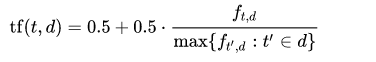
\includegraphics[width=0.5\linewidth]{tf.png}
%	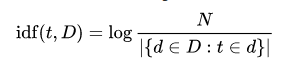
\includegraphics[width=0.5\linewidth]{idf.png}
		\subsection{POS-tagging} \label{l2}
		\begin{frame} %\label{l4}
			\frametitle{\insertsection}
			\frametitle{\insertsubsection}
			\begin{itemize}
				\item \textbf{Lexical Based Methods} — Assigns the POS tag the most frequently occurring with a word in the training corpus
				\item \textbf{Rule-Based Methods} — Assigns POS tags based on rules. For example, we can have a rule that says, words ending with “ed” or “ing” must be assigned to a verb. Rule-Based Techniques can be used along with Lexical Based approaches to allow POS Tagging of words that are not present in the training corpus but are there in the testing data.
		\end{itemize}
\end{frame}


\begin{frame} %\label{l4}
	\frametitle{\insertsection}
	\frametitle{\insertsubsection}
	\begin{itemize}
		\item \textbf{Probabilistic Methods} — This method assigns the POS tags based on the probability of a particular tag sequence occurring. Conditional Random Fields (CRFs) and Hidden Markov Models (HMMs) are probabilistic approaches to assign a POS Tag.
		\item \textbf{Deep Learning Methods} — Recurrent Neural Networks can also be used for POS tagging.
	\end{itemize}
\end{frame}


	

\begin{frame} %\label{l4}
	\frametitle{\insertsection}
	\frametitle{\insertsubsection}

	
	\vspace{0.5cm}
	
	\begin{itemize}
		\item "I LOVE you, honey" { } vs. "Lets make LOVE, honey"
		\item Text to Speech Conversion
		
		\vspace{0.5cm}
		
		 \textcolor{red}{They \emph{refuse} to permit us to obtain the \emph{refuse} permit.}
	%	\item \text{refUSE (/rəˈfyo͞oz/) V}
	
	\vspace{0.5cm}
	
		\item refUSE  (/r\textschwa 'fy$\overline{oo}$z/) V
		\item refUSE  (/refy,$\overline{oo}$s/) N
	%	\item \text{REFuse(/ˈrefˌyo͞os/) N}
	\end{itemize}
\end{frame}	



\begin{frame} %\label{l4}
	\frametitle{\insertsection}
	\frametitle{\insertsubsection}
	
	
	\vspace{0.5cm}
	
	\begin{itemize}
		\item Noun (N)- Daniel, London, table, dog, teacher, pen, city, happiness, hope

		\item Verb (V)- go, speak, run, eat, play, live, walk, have, like, are, is

		\item Adjective(ADJ)- big, happy, green, young, fun, crazy, three
	\item Adverb(ADV)- slowly, quietly, very, always, never, too, well, tomorrow
	\item Preposition (P)- at, on, in, from, with, near, between, about, under
	\item Conjunction (CON)- and, or, but, because, so, yet, unless, since, if
	\item Pronoun(PRO)- I, you, we, they, he, she, it, me, us, them, him, her, this
	\item Interjection (INT)- Ouch! Wow! Great! Help! Oh! Hey! Hi!
	\end{itemize}
\end{frame}	

\subsection{Chunking}
    \begin{frame} %\label{l4}
    	\frametitle{\insertsection}
    	\frametitle{\insertsubsection}
    	
    	the little yellow dog barked at the cat
    	
    	\vspace{0.5cm}
    	
    	REGEX  =  \textcolor{red}{NP: {<DT>?<JJ>*<NN>} } 
    	
    	\vspace{0.5cm}
    	
 		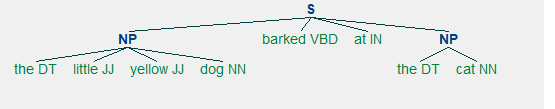
\includegraphics[width=0.7\linewidth]{ch.png}
 		
 		\vspace{0.5cm}
 		
 	\textcolor{black}{\small{\href{https://pythonprogramming.net/chunking-nltk-tutorial/}{check NLTK page}} }
    
	\end{frame}	

\subsection{Lexical distances}
    \begin{frame} %\label{l4}
	\frametitle{\insertsection}
	\frametitle{\insertsubsection}
	 
		 Levenshtein distance
	
	\begin{itemize}
		\item sitten \MVRightarrow { }sittin
		\item kitten \MVRightarrow { }sitten
		\item sittin \MVRightarrow { }sitting 
	\end{itemize}
	
\end{frame}	% Jaccard Similarity

    \begin{frame} %\label{l4}
	\frametitle{\insertsection}
	\frametitle{\insertsubsection}
	
	Jaccard Similarity
	
	\begin{itemize}
		\item Sentence 1: AI is our friend and it has been friendly
		\item Sentence 2: AI and humans have always been friendly
	\end{itemize}
	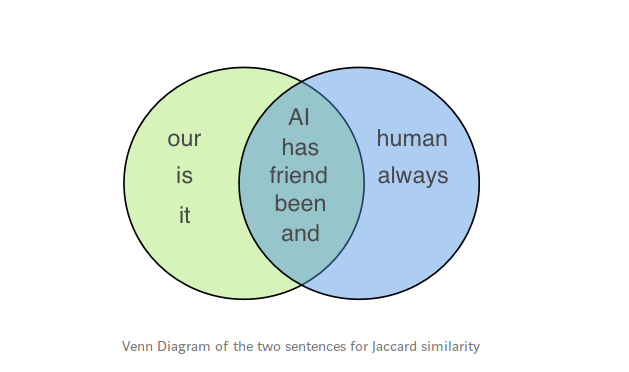
\includegraphics[width=0.7\linewidth]{jac.png}
\end{frame}	% 

    \begin{frame} %\label{l4}
	\frametitle{\insertsection}
	\frametitle{\insertsubsection}
	
	Cosine distance
	
	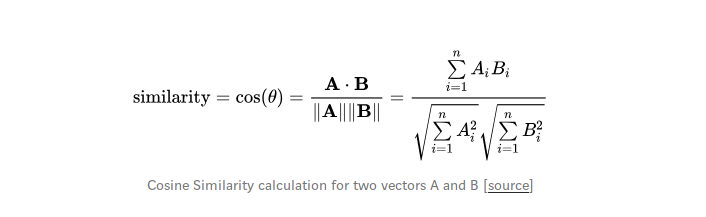
\includegraphics[width=0.9\linewidth]{cos.png}
\end{frame}	% 


\end{document}